\documentclass[12pt]{article}
\usepackage[utf8]{inputenc}
%\usepackage[T1,T2A]{fontenc}
\usepackage[T2A]{fontenc}
\usepackage[serbian]{babel}
\usepackage{geometry}
\geometry{margin=1in}
%\usepackage{helvet}
%\usepackage{avant}
\renewcommand{\familydefault}{\sfdefault}
\usepackage{graphicx}
\usepackage{multicol}
\usepackage[document]{ragged2e}
\usepackage{fancyhdr}
\usepackage{hyperref}
\usepackage[svgnames]{xcolor}
\usepackage{caption}
\usepackage{float}
\usepackage{subcaption}

\usepackage{tocloft}
\renewcommand{\cftsecleader}{\cftdotfill{\cftdotsep}}

%\newcommand{\mycode}[1]{\texttt{\colorbox{LightGrey}{#1}}}
\newcommand{\mycode}[1]{\texttt{\colorbox{Lavender}{#1}}}

\hypersetup{
    colorlinks=true,
    linkcolor=black,
    filecolor=black,      
    urlcolor=blue,
    }

\pagestyle{fancy}
\fancyhf{}
\fancyhead[L]{Програмирање мобилних апликација}
%\fancyhead[C]{Top Center}
\fancyhead[R]{документација}
\renewcommand{\headrulewidth}{0.4pt}
%\fancyfoot[L]{Bottom Left}
\fancyfoot[C]{\thepage}
%\fancyfoot[R]{Bottom Right}
\renewcommand{\footrulewidth}{0.4pt}

\addto\captionsserbian{\renewcommand*\contentsname{Садржај:}}
%\setcounter{tocdepth}{2}
\addto\captionsserbian{\renewcommand{\figurename}{Слика}}

%\setlength\parindent{24pt}

\begin{document}
\thispagestyle{empty}
\begin{center}
\Large{
Универзитет у Крагујевцу
\vspace{0.3cm}\\
Факултет инжењерских наука
}
\vspace{0.7cm}\\

\includegraphics{images/fin_image}
\vspace{0.7cm}\\
\LARGE{
\textbf{Предмет:}
\vspace{0.1cm}\\
Програмирање мобилних апликација
}
\vspace{1cm}\\
\LARGE{
\textbf{Тема:}
\vspace{0.1cm}\\
Мобилна апликација за даљинско управљање бравом улазних врата и осветљењем у просторијама куће
}
\vspace{2cm}
\end{center}

\begin{tabular}{l}
\textbf{Студенти:}\\
Вељко Максимовић 634/2018\\
Ђорђе Гачић 626/2018\\
\end{tabular}
\setlength{\tabcolsep}{12em}
\begin{tabular}{l}
\textbf{Професор:}\\
Др Ненад Грујовић\\
\vspace{0.02cm}\\
\textbf{Асистент:}\\
Вукашин Славковић, дипл. маш. инж.\\
\end{tabular}
\begin{center}
\vspace{1cm}
Крагујевац, фебруар 2022.
\end{center}
\newpage

\tableofcontents
\newpage

\section{Увод}
\justifying
У данашње време, када су мобилни телефони и остали паметни уређаји свакодневно присутни у животу просечног човека, отварају се разне могућности за њихову употребу у многим сферама живота. Паметни телефони данас имају многе функције и, ако се на исправан начин употребљавају, могу много да олакшају живот и разне послове. Поред уобичајене употребе за размену позива и порука тј. за комуникацију уопште, паметни телефони се користе и за забаву, оријентацију у простору, фотографисање, снимање видео материјала, мобилно банкарство, праћење разних параметара и догађаја, опште и научно информисање као и уопштено за приступ Интернету. Поред свега наведеног, све више улазе у примену мобилне апликације које бежично (даљински) управљају (Wi-Fi, Bluetooth итд.) неким физичким уређајима или електронским компонентама. Једна од примена тих апликација јесте и у домаћинству како би се контролисао рад многих уређаја као нпр. кућни апарати (шпорети, фрижидери, веш машине), сијалице, браве итд.
\vspace{0.3cm}\\\indentУ овом пројекту је реализована једна таква апликација чија је функција управљање целокупним осветљењем и бравом на улазним вратима куће. У оквиру пројекта су, поред саме апликације, физички присутне и уграђене све електронске компоненте које симулирају поменуте процесе, а израђена је и макета куће како би функционалност апликације била веродостојније приказана. 
\vspace{0.3cm}\\\indentМотивација за израду овог пројекта била је идеја да се повећа сигурност домаћинства тако што ће контрола неких његових делова бити на пар кликова од самог корисника. Тако бисмо преко неколико кликова могли бити сигурни да су сва светла у кући угашена и да су улазна врата закључана без да идемо да проверавамо. Такође, ова апликација представља само део могућности које пружа технологија тзв. паметних домова (енг. Smart Home) и очекује се са у будућности мобилне апликације тог типа буду у свакодневној употреби код већине људи.\\

\newpage
\section{Потребе реалног система}
\justifying
Имплеменација реалног система на тему даљинског управљања бравом и осветљењем у домаћинсву је прилично захтевна због великог броја компоненти које се морају уклопити у једну практичну и функционалну целину.
\vspace{0.3cm}\\\indentРеални систем захтева следеће компоненте:
\begin{itemize}
  \item Паметни уређај (паметни телефон, таблет, ...)
  \item Светлосна група - осветљење у свим просторијама
  \item Систем закључавања који подржава даљинско управљање
  \item Мотор који покреће систем закључавања
  \item Уређај за остваривање даљинске везе
  \item Микроконтролерски уређај за управљање целокупним системом
  \item Напајање за целокупни систем
  \item Ожичење целокупног система
\end{itemize}
\vspace{0.3cm}
\indent\indentРеални систем може захтевати још много помоћних компоненти али, с обзиром да се пројектни задатак односи само на прототип једног таквог система, задржаћемо се на горе набројаним компонентама. У наредним поглављима ће бити детаљно приказан начин на који су поменуте компоненте уграђене у прототип система као и које су компоненте у питању. Такође ће бити детаљно објашњен начин на који је имплементирана сама мобилна апликација - софтверска реализација пројекта.

\newpage
\section{Опис коришћене технологије и компоненти}
\subsection{Опис хардверских компоненти}
\indentМикроконтролерски уређај за управљање прототипом система је \href{https://store.arduino.cc/products/arduino-uno-rev3}{Arduino Uno R3}. То је микроконтролерска плоча заснована на \href{http://ww1.microchip.com/downloads/en/DeviceDoc/Atmel-7810-Automotive-Microcontrollers-ATmega328P\_Datasheet.pdf}{ATmega328P}. Има 16 дигиталних улазно/излазних пинова, 6 аналогних улаза, USB конекцију, прикључак за напајање итд. Садржи све што је потребно за подршку микроконтролеру. Уређај се преко USB кабла повезује на рачунар да би се испрограмирао при чему се и напаја преко истог кабла. Ако је потребно само напајање оно се, поред поменутог начина, може остварити и AC-DC адаптером или батеријом. 
%\begin{figure}[h]
   % \centering
   % 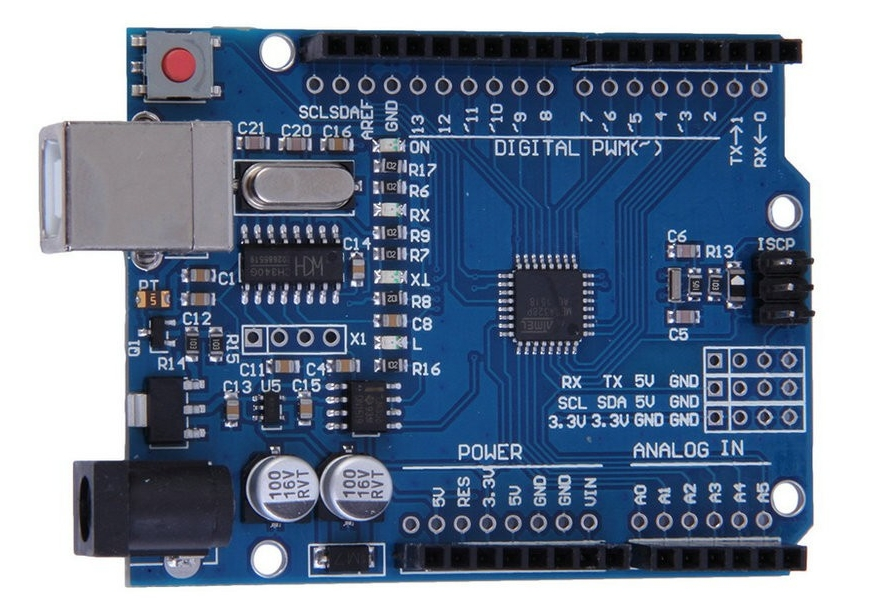
\includegraphics[height=6cm, width=10cm]{images/arduino}
   % \caption{Arduino Uno R3}
   % \label{Image 1:}
%\end{figure}
\begin{center}
    \centering 
    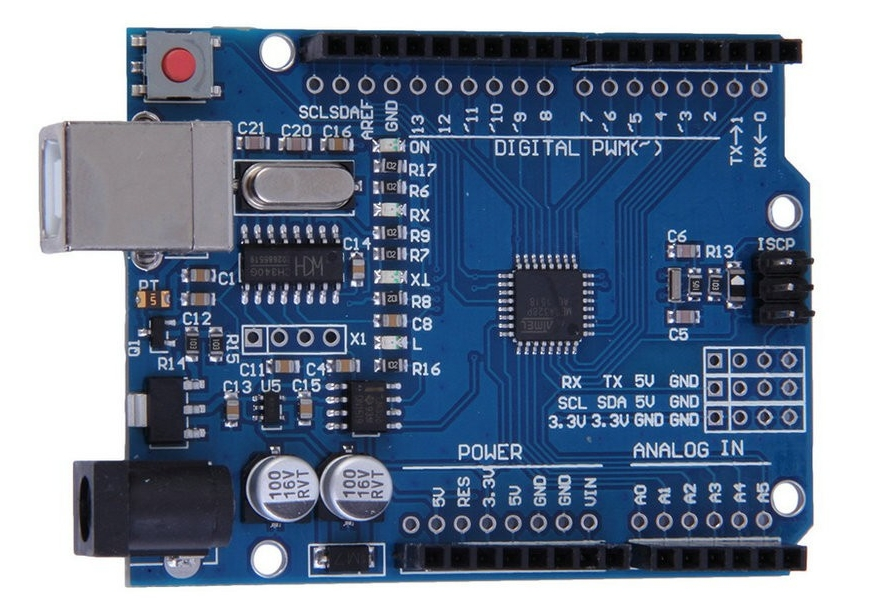
\includegraphics[height=7cm, width=10cm]{images/arduino}
     \captionof{figure}{Arduino Uno R3}
\end{center}
\vspace{0.5cm}
\indent\indentУређај за остваривање даљинске (бежичне) везе је \href{https://components101.com/sites/default/files/component\_datasheet/HC-05\%20Datasheet.pdf}{HC-05 bluetooth модул} и представља једноставан за коришћење Bluetooth SPP (Serial Port Protocol) модул. Преко њега се може остварити двосмерна бежична функционалност тј. може се користити и као 'master' и као 'slave'. У оквиру овог пројекта користиће се само као 'slave' јер ће наредбе ићи само од апликације ка модулу а не и обрнуто. 
\vspace{0.5cm}
\begin{center}
    \centering 
    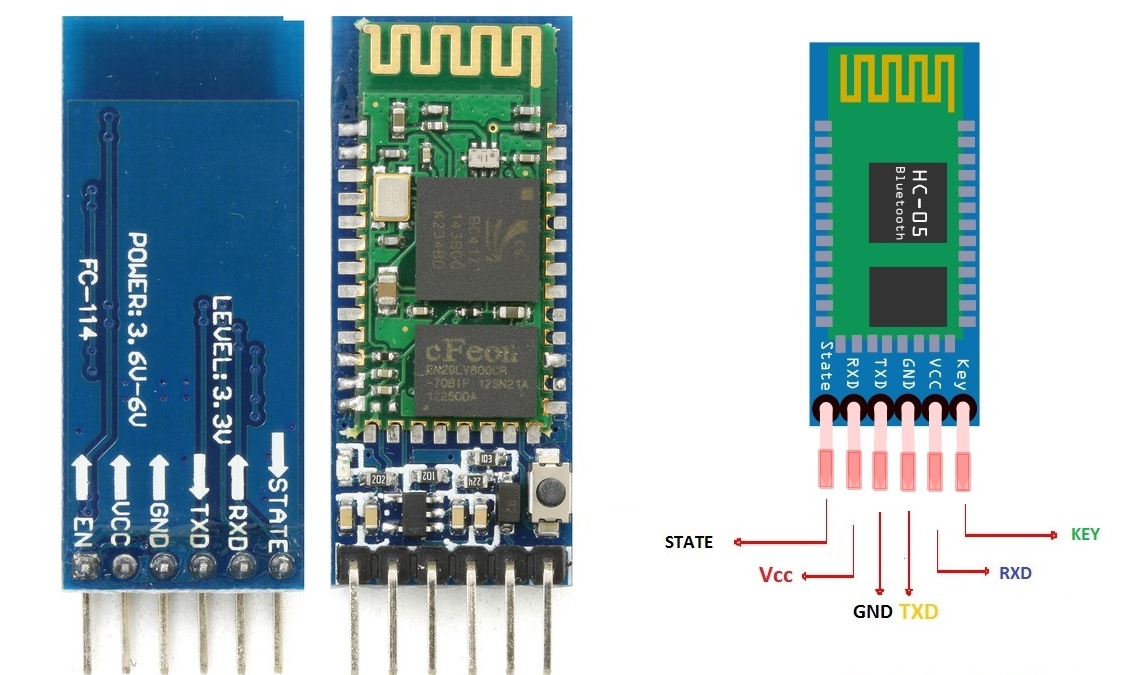
\includegraphics[height=5cm, width=10cm]{images/hc-05}
     \captionof{figure}{HC-05 bluetooth модул}
\end{center}
\vspace{0.5cm}
\indent\indentСветлосну групу у прототипу система чиниће шест светлећих диода (\href{https://en.wikipedia.org/wiki/Light-emitting_diode}{LED} - Light Emitting Diode) црвене боје које ће да представљају осветљење у просторијама.
\vspace{0.5cm}
\begin{center}
    \centering 
    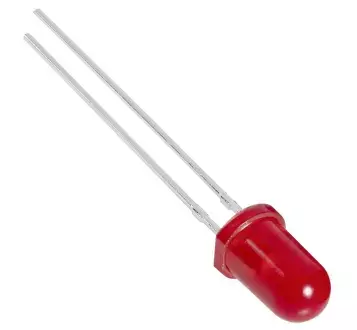
\includegraphics[height=3cm, width=3cm]{images/led}
     \captionof{figure}{LED}
\end{center}
\vspace{0.5cm}
%\begin{itemize}
%  \item Дневни боравак (Living Room)
%  \item Спаваћа соба (Bedroom)
%  \item Дечија соба (Children's Room)
%  \item Кухиња (Kitchen)
%  \item Купатило (Bathroom)
%  \item Ходник (Hallway)
%\end{itemize}
\indent\indentМотор који покреће систем закључавања браве у овом пројекту је серво мотор (\href{http://www.ee.ic.ac.uk/pcheung/teaching/DE1_EE/stores/sg90_datasheet.pdf}{Micro Servo SG90}) са једнокраким пропелером. Серво мотори су мотори високог обртног момента који се обично користе у роботици и неким другим апликацијама због чињенице да је лако контролисати њихову ротацију. Серво мотори имају зупчасту излазну осовину која се може електронски контролисати. Због контроле, за разлику од обичних DC мотора, серво мотори обично имају додатни пин поред два пина за напајање (VCC и GND) који је сигнални пин. Сигнални пин се користи за контролу серво мотора, окрећући његову осовину под било којим жељеним углом.
\begin{center}
    \centering 
    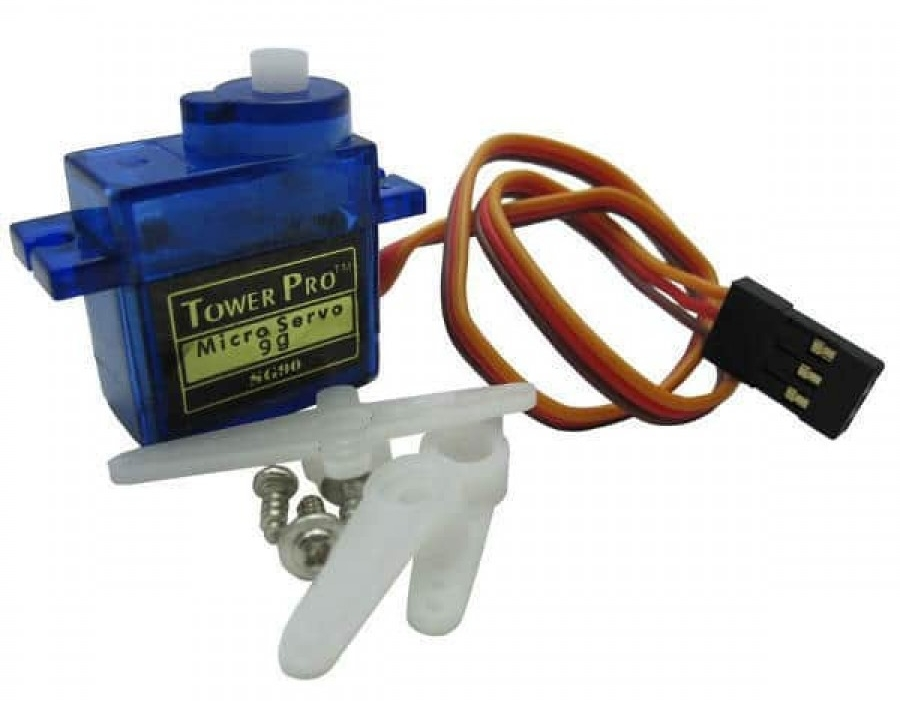
\includegraphics[height=5cm, width=7cm]{images/servo}
     \captionof{figure}{Micro Servo SG90}
\end{center}
\vspace{0.5cm}
\indent\indentЗа ожичење су коришћене краткоспојне жице са конекторима следећих типова:
\begin{itemize}
  \item Female to Female
  \item Male to Female
  \item Male to Male
\end{itemize}
\begin{figure}[H]
\centering
\subcaptionbox{Male to Female}{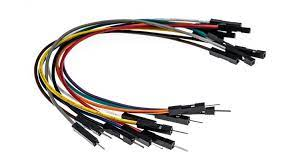
\includegraphics[height=4cm, width=5cm]{images/wires1}}
\hfill % <-- Seperation
\subcaptionbox{Female to Female}{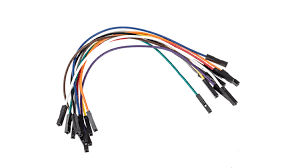
\includegraphics[height=5cm, width=6cm]{images/wires2}}
\hfill % <-- Seperation
\subcaptionbox{Male to Male}{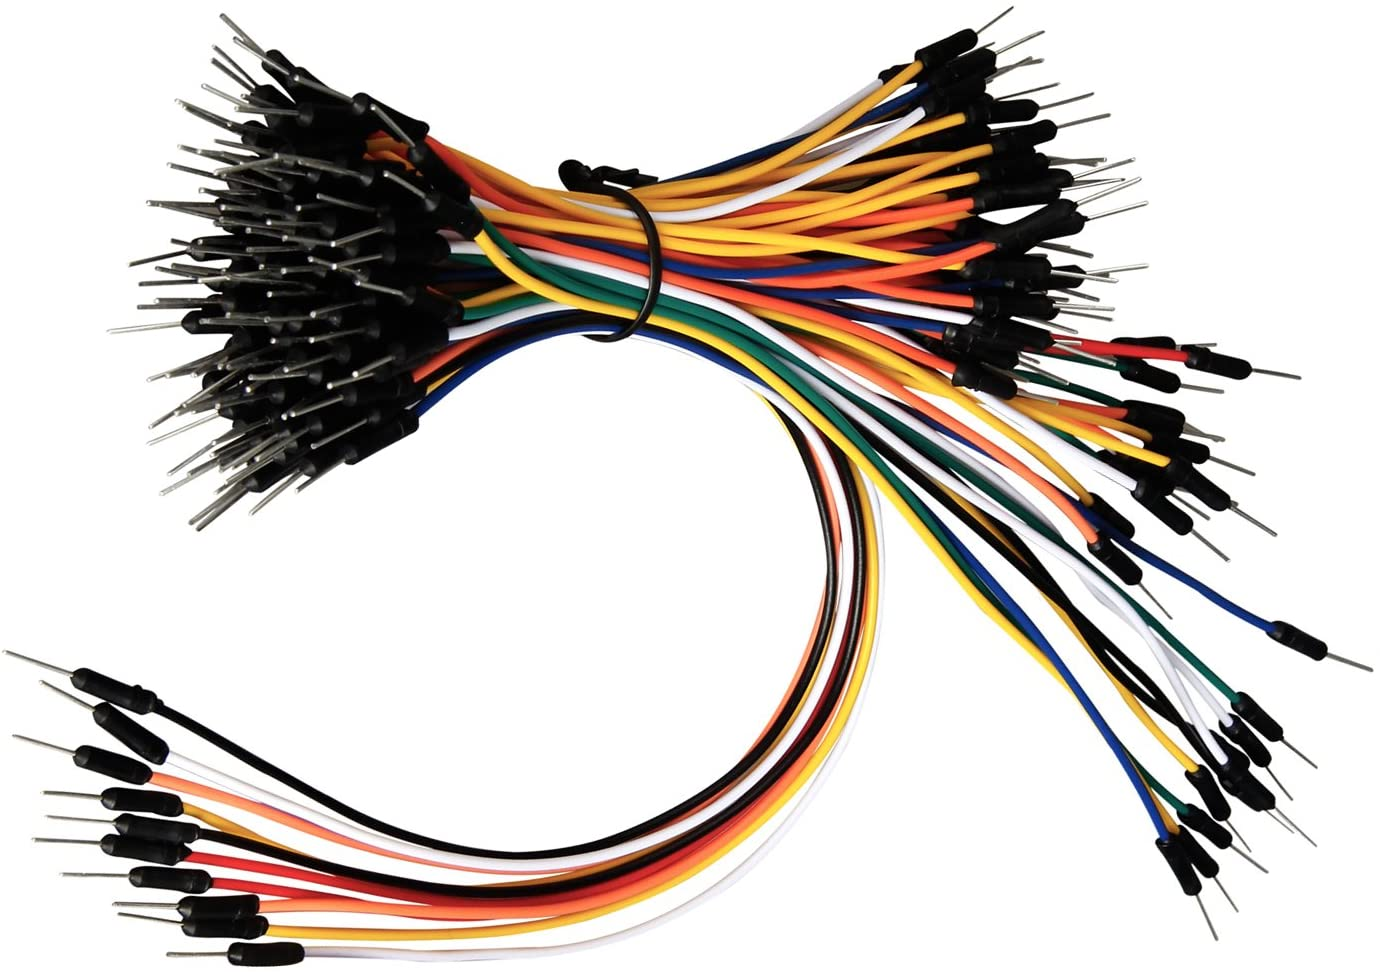
\includegraphics[height=4cm, width=5cm]{images/wires3}}
\caption{Жице са различитим комбинацијама конектора}
\end{figure}
\vspace{0.2cm}
\indent\indentЗа напајање се у оквиру реализованог пројекта користе батерија од 9 волти за напајање Arduino плоче и лежиште са три батерије од по 1.5 волти (тип AA) за напајање серво мотора, с тим да се у току реализације за напајање Arduino плоче користио USB каонектор преко кога се одвијало и програмирање микроконтролера.
\vspace{0.5cm}
\begin{center}
    \centering 
    \includegraphics[height=7cm, width=15cm]{images/power}
     \captionof{figure}{Напајање: 3xAA 1.5V, 9V, USB конектор}
\end{center}
\vspace{0.5cm}
\indent\indentКао простор за повезивање коришћена је прото плоча (енг. \href{http://www.busboard.com/documents/datasheets/BPS-DAT-(BB830)-Datasheet.pdf}{breadboard}) са 830 пинова. Једна таква је приказана на следећој слици:
\begin{center}
    \centering 
    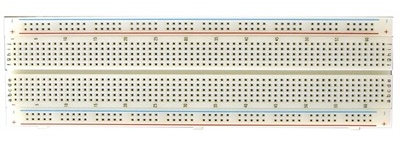
\includegraphics[height=5cm, width=13cm]{images/breadboard}
     \captionof{figure}{Прото плоча}
\end{center}
\vspace{0.5cm}
\indent\indentПаметни уређај на коме је инсталирана мобилна апликација у оквиру овог пројекта је паметни телефон са Android оперативним системом. Међутим, мобилна апликација у оквиру овог пројекта је имплементирана у Flutter мулти-платформском окружењу које омогућава израду апликација независно од оперативног система на коме се инсталира апликација, тако да би реализована апликација требала радити и на другим оперативним системима за паметне уређаје (нпр. iOS). \vspace{0.3cm}\\ 
\indentПретходно су приказане све компоненте које се налазе у хардверском делу реализованог пројекта и све се могу наћи у слободној продаји. Начин повезивања свих компоненти биће објашњен и илустративно приказан у поглављу које се односи на сам начин реализације целокупног пројекта.

\subsection{Софтверске потребе пројекта}
У наставку ће бити набројани софтверски алати, радна окружења као и програмски језици који су били неопходни за реализацију читавог пројекта:
\begin{itemize}
  \item \href{https://www.arduino.cc/en/software}{Arduino IDE 1.8.19} софтвер који омогућава компајлирање кода за Arduino и такође његово учитавање на плочу (енг. upload). Софтвер је бесплатан и доступан за све оперативне системе (Windows, Linux, Mac OS).
  \item \href{https://en.wikipedia.org/wiki/C_(programming_language)}{C програмски језик} - језик у коме се пише код за програмирање микроконтролера на Arduino плочи.
  \item \href{https://en.wikipedia.org/wiki/Flutter\_(software)}{Flutter} - оквир за развој софтвера отвореног кода. Креиран је од стране Google-а. Користи се за развој мулти-платформских апликација за Android, iOS, Linux, Mac, Windows и интернет апликација (Web) и то из једне исте базе кода. Инсталација самог окружења је такође доступна за више оперативних система, а сам поступак инсталације и кораци који треба да се прате најбоље су објашњени у званичној Flutter \href{https://docs.flutter.dev/get-started/install}{документацији}.
  \item \href{https://en.wikipedia.org/wiki/Dart\_(programming\_language)}{Dart програмски језик} - језик који користи Flutter и у коме се пише код саме апликације. Инсталира се заједно са Flutter окружењем. Развио га је Google и намењен је развоју клијентских апликација, као што су интернет и мобилне апликације, а може се користити и за израду сервер и десктоп апликација. У наредном поглављу биће приказани и објашњени поједини делови кода писаног у Dart програмском језику за потребе апликације у оквиру нашег пројекта.
  \item \href{https://code.visualstudio.com/}{Visual Studio Code} - уређивач изворног кода који је развио Microsoft за Windows, Linux i Mac OS. Софтвер је бесплатан и слободан за приватну или комерцијалну употребу. У нашем пројекту је коришћен за писање кода у оквиру Flutter окружења које се веома једноставно подешава за VS Code ако се прате \href{https://docs.flutter.dev/get-started/editor?tab=vscode}{инструкције} које се такође налазе у оквиру званичне Flutter документације.
  \item \href{https://en.wikipedia.org/wiki/LaTeX}{Latex} - коришћен за израду документације нашег пројекта. Представља описни језик и систем за припрему докумената. Latex је у широкој употреби у академији, а користи се за објављивање научних докумената у многим областима, укључујући математику, физику, информатику, статистику, економију, и политичке науке. Може се преузети са званичног \href{https://www.latex-project.org/get/}{сајта}, а може се користити и онлајн Latex уређивач при чему не мора да се инсталира на рачунар. За израду ове документације коришћен је онлајн уређивач који се назива \href{https://www.overleaf.com/project}{Overleaf} и пружа заиста сјајан и прилагођен интерфејс и брзину генерсања документа.
  \item \href{https://www.tinkercad.com/dashboard}{Tinkercad} - онлајн уређивач који је у оквиру овог пројекта коришћен за цртање шеме повезивања хардверских компоненти. Све што је потребно јесте направити налог на овом сајту.
\end{itemize}



\newpage
\section{Начин повезивања хардверских компоненти}
\indentУ претходном поглављу набројане су и описане све коришћене хардверске компоненте. У наставку ће бити приказана шема повезивања тих компоненети како би представљале функционалну целину када се изради апликација.    
\begin{center}
    \centering 
    \includegraphics[height=12cm, width=17cm]{images/sema\_tinkercad}
     \captionof{figure}{Шема са сликовитим приказом компоненти}
\end{center}
\vspace{0.5cm}
\indent\indentНа претходној шеми је приказан исправан начин повезивања компоненти. На шеми недостаје 9V батерија која напаја Arduino плочу, али је ту USB конектор који врши исту функцију. Разлог изосатвљања батерије јесте немогућност уређивача да прикаже Arduino плочу без USB конектора. Из сличног разлога је серво мотор приказан са пропелером који има два крака, а не један како је предвиђено у списку компоненети. Светлећих диода има шест и свака ће, како је већ поменуто, да служи као осветљење за једну просторију. То значи да је предвиђено да има шест просторија у макети куће, а оне су следеће:
\begin{itemize}
  \item Дневни боравак (Living Room)
  \item Спаваћа соба (Bedroom)
  \item Дечија соба (Children's Room)
  \item Кухиња (Kitchen)
  \item Купатило (Bathroom)
  \item Ходник (Hallway)
\end{itemize}
\vspace{0.5cm}
\indent\indentСледи поједностављен приказ шеме на коме се јасно види види логика повезивања електронских компоненети. Шема је израђена помоћу \href{https://easyeda.com/}{EasyEda} онлајн уређивача за шеме електронских компоненти (слично као Tinkercad али на нижем нивоу када је у питању изглед компоненти). Треба напоменути да и Tinkercad и EasyEda могу да послуже као симулатори електронских склопова, али су у оквиру овог пројекта коришћени само за израду шеме у циљу појашњења начина повезивања компоненти и нису рађене симулације.
\begin{center}
    \centering 
    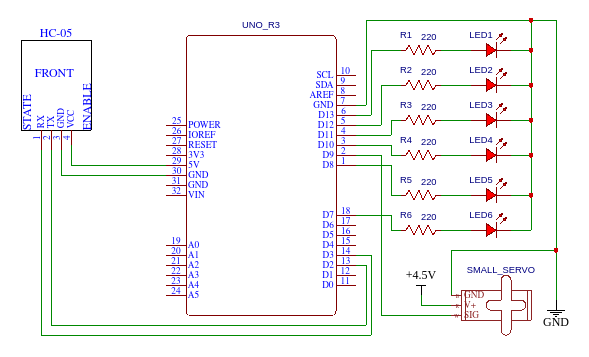
\includegraphics[height=10cm, width=15cm]{images/sema_easyeda.png}
     \captionof{figure}{Поједностављен приказ шеме}
\end{center}
\vspace{0.5cm}
\indent\indentУ следећем приказу (фотографија) јесте повезана шема свих реалних хардверских компоненети које су у саставу овог пројекта.
\begin{figure}[H]
\centering
\subcaptionbox{Приказ одозго}{\includegraphics[height=12cm, width=16cm]{images/sema-foto1}}
\vspace{0.5cm}\\
%\hfill % <-- Seperation
\subcaptionbox{Приказ спреда}{\includegraphics[height=5cm, width=8cm]{images/sema-foto2}}
\hfill % <-- Seperation
\subcaptionbox{Приказ - укључено}{\includegraphics[height=5cm, width=8cm]{images/sema-foto3}}
\caption{Фотографијe израђене шеме повезивања компоненети}
\end{figure}


\newpage
\section{Софтверска реализација пројекта}
\subsection{Програмирање мокроконтролера}
Како је већ речено, програмирање микроконтролера на Arduino плочи вршимо у окружењу Arduino IDE у програмском језику C. Код се налази у \texttt{light\_and\_lock\_arduino\_code.ino} датотеци. Да би се код учитао на Arduino потребно је повезати га са рачунаром помоћу USB конектора. Након покретања Arduino IDE окружења потребно је извршити следећа подешавања:
\begin{itemize}
    \item Селектовати \texttt{Tools > Board} и одабрати \texttt{Arduino Uno}.
    \item Селектовати \texttt{Tools > Port} и одабрати USB порт на који је прикључен Arduino преко USB конектора (и нашем случају је то \texttt{/dev/ttyUSB0}).
\end{itemize}
\indentУ наставку ће бити објашњени најбитнији делови изворног кода:
\begin{center}
    \centering 
    \includegraphics[height=8cm, width=8cm]{images/arduino\_code1}
     \captionof{figure}{Arduino изворни код 1}
\end{center}
\indent\indentНа самом почетку потребно је учитати библиотеку \texttt{\href{https://www.arduino.cc/en/Reference/softwareSerial}{SoftwareSerial}} која омогућава серијску комуникацију са апликацијом, као и библиотеку \texttt{\href{https://www.arduino.cc/reference/en/libraries/servo/}{Servo}} која омогућује управљање серво мотором. Након тога декларишемо Bluetooth везу тако што Arduino пиновe 2 и 3 доделимо за TX и RX конекторе bluetooth модула, респективно. Затим се декларише променљива за серво мотор која је типа \texttt{Servo}. Променљива \texttt{incomingByte} типа \texttt{char} се користи да би се пријемни податак (наредба која долази са паметног уређаја) сместила унутар ове променљиве. Затим следе променљиве типа \texttt{int} помоћу којих касније дефинишемо које пинове развојног окружења користимо као излазне параметре. Помоћу њих вршимо контролу управљаних догађаја (осветљење и управљање бравом). Променљива \texttt{pos} је предвиђена за позицију серво мотора. \\
\indentЗатим следи мотода \texttt{setup} која се позива само једном и то при извршавању кода тј. учитавању на Arduino:
\begin{center}
    \centering 
    \includegraphics[height=8cm, width=12cm]{images/arduino\_code2}
     \captionof{figure}{Arduino изворни код 2 - \texttt{setup} метода}
\end{center}
\indent\indentУнутар методе \texttt{setup} позивају се \texttt{pinMode} функције преко којих се претходно дефинисани пинови означавају као излазни. Такође, врши се повезивање контроле серво мотора на пин предвиђен за то преко функције \texttt{attach}, а то је пин 9. Након тога позива се функција \texttt{digitalWrite} којом се на све пинове који ће да се користе шаље низак напон као почетна конфигурација. На крају се поставља и иницијализује серијска bluetooth комуникација као њена брзина која је изражена у \texttt{\href{https://en.wikipedia.org/wiki/Baud}{baud rate}}-овима.
\vspace{0.5cm}\\
\indentСледи функција \texttt{loop} која се позива стално након учитавања кода на Arduino, наравно све док се напајање не прекине и по томе се разликује од \texttt{setup} функције која се позива само једном.
\begin{center}
    \centering 
    \includegraphics[height=8.5cm, width=10cm]{images/arduino\_code3}
\end{center}
\begin{center}
    \centering 
    \includegraphics[height=9cm, width=10cm]{images/arduino\_code4}
     \captionof{figure}{Arduino изворни код 3 - \texttt{loop} метода}
\end{center}
\indent\indentУнутар методе \texttt{loop} се на почетку преко функције \texttt{available} проверава да ли је број бајтова (карактера) доступних за читање преко софтверског серијског порта већи од 0. Ако јесте, тај карактер се чита преко функције \texttt{read} и смешта у променљиву \texttt{incomingByte} и то ће нам представљати податак који је послат од стране мобилне апликације тј. 'master'-а ка bluetooth модулу тј. 'slave'-у. Затим се врши провера који је то карактер. \\
\indentЗа потребе овог пројекта усвојени су карактери од \texttt{'а'} до \texttt{'n'} по абецедном реду. Логика је та да нпр. ако стигне наредба 'а', преко функције \texttt{digitalWrite} се на пин који је предвиђен за контролу осветљења у дневном боравку (\texttt{LivingRoomPin}) шаље висок напон чиме се диода засветли, и светли све док не стигне низак напон на тај исти пин. Низак напон на тај исти пин стиже кад стигне наредба 'b'. Исти процес се одвија за све остале пинове који су задужени за осветљење само се шаљу други карактери као наредбе.\\
\indentОно што се разликује јесте како се реагује на наредбе 'm' и 'n' које служе као наредбе да се покрене серво мотор тј. да се откључа брава ако је примљена наредба 'm', а да се закључа ако је примљена наредба 'n'. Ако се прими било која од ове две наредбе, поставља се висок напон на пин који је предвиђен за контролу серво мотора (\texttt{servoPin}). Затим следи постављање жељене вредности за позицију пропелера серво мотора преко функције \texttt{\href{https://www.arduino.cc/reference/en/language/functions/math/map/}{map}}. Након тога се преко функције \texttt{write} подешава позиција серво мотора и шаље се низак напон на \texttt{servoPin}.
\vspace{0.3cm}\\
\indentКада се заврши са програмирањем, треба изабрати опцију \texttt{Sketch > Verify/Compile} што ће покренути процес компајлирања кода и уједно га верификовати (проверти да ли је исправан). Ако је код исправан, одради се следећи поступак: одабере се \texttt{Sketch > Upload}, чиме се код учита тј. инсталира на микроконтролерску плочу (Arduino Uno) и тиме је процес програмирања микроконтролера за овај проекат завршен.


\subsection{Програмирање мобилне апликације}
\indentКао што је већ поменуто, мобилна апликација је израђена у Flutter окружењу при чему се користио Visual Studio Code уређивач текста. Након подешавања Flutter окружења у VS Code-у потребно је направити празан Flutter пројекат (апликацију) по \href{https://docs.flutter.dev/get-started/test-drive?tab=vscode}{упутству} из документације.\\ 
\indentПри изради пројекта апликација је тестирана на Android паметном телефону. За инсталацију апликације на уређају је потребан USB кабл који ће да повезује рачунар и паметни телефон. Да би се проверило да ли Flutter препознаје уређај потребно је отићи на терминал у оквиру VS Code окружења, ући у директоријум пројекта (у нашем случају назив пројекта је \texttt{light\_and\_lock\_bluetooth\_control\_flutter\_app}) и унети команду \texttt{flutter devices}. Ако на стандардном излазу испише конектовани уређај, значи да ће апликација моћи да се инсталира уколико нема грешке. Да би се апликација инсталирала потребно је унети команду \texttt{flutter run}.\\
\indentДа би реализована апликација радила радила исправно, потребно је извршити подешавања у две датотеке. То су \texttt{android/app/build.gradle} где је потребно пронаћи \texttt{defaultConfig} секцију и подесити \texttt{minSdkVersion} на 19:
\begin{center}
    \centering 
    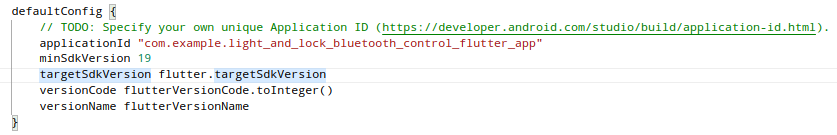
\includegraphics[height=3.5cm, width=16cm]{images/defaultConfigBuildGradle}
     \captionof{figure}{Модификација \texttt{build.gradle} датотеке}
\end{center}
\indent\indentНакон тога је потребно креирати \texttt{images} директоријум унутар директоријума Flutter пројекта и у њега убацити слике које ће се користити при изради графичког интерфејса апликације:
\begin{figure}[H]
\centering
\subcaptionbox{light\_off.png}{\includegraphics[height=5cm, width=3cm]{images/light\_off.png}}
\hfill % <-- Seperation
\subcaptionbox{light\_on.png}{\includegraphics[height=5cm, width=3cm]{images/light\_on.png}}
\hfill % <-- Seperation
\subcaptionbox{locked.png}{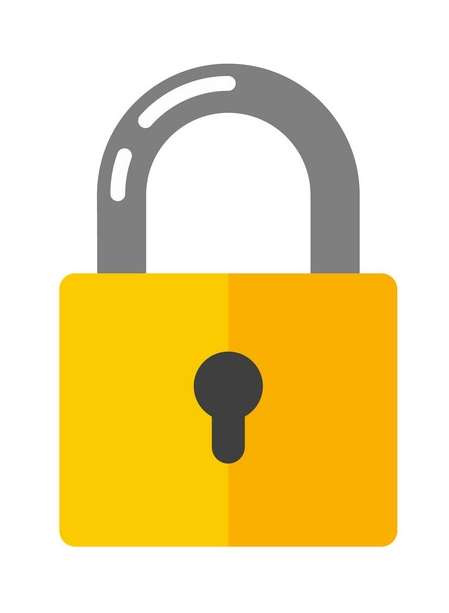
\includegraphics[height=4cm, width=3cm]{images/locked.png}}
\hfill % <-- Seperation
\subcaptionbox{unlocked.png}{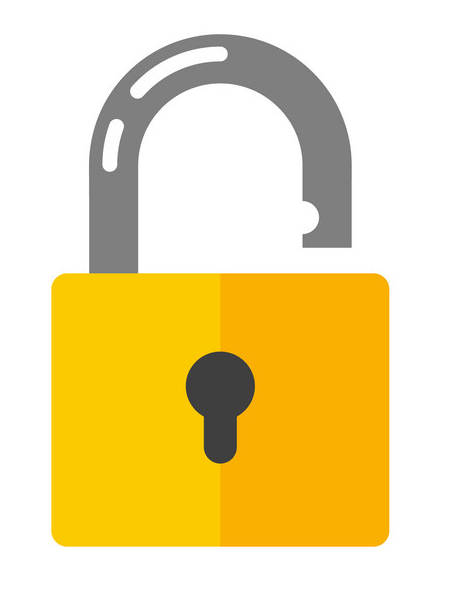
\includegraphics[height=4cm, width=3cm]{images/unlocked.png}}
\vspace{0.3cm}
\caption{Илустрације потребне за израду графичког интерфејса апликације}
\end{figure}
\indentДа би се слике исправно учитале потребно је отворити \texttt{pubspec.yaml} датотеку и у њој пронаћи \texttt{flutter: assets:} секцију и додати путање до слика као на примеру испод:
\begin{center}
    \centering 
    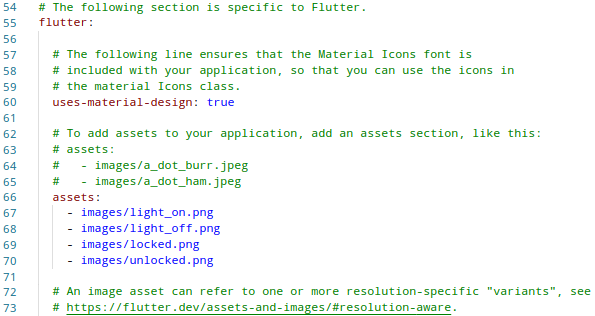
\includegraphics[height=7cm, width=12cm]{images/assets}
     \captionof{figure}{Модификација \texttt{pubspec.yaml} датотеке - учитавање слика}
\end{center}
\indent\indentПоред тога, у \texttt{pubspec.yaml} датотеци потребно је пронаћи секцију \texttt{dependencies:} и додати зависности за bluetooth серијску комуникацију и Toast поруке:
\begin{center}
    \centering 
    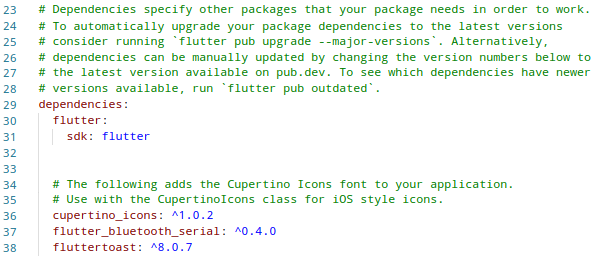
\includegraphics[height=6cm, width=12cm]{images/dependencies}
     \captionof{figure}{Модификација \texttt{pubspec.yaml} датотеке - dependencies}
\end{center}
\vspace{0.3cm}
\indent\indentНајбитнија датотека у којој се пише комплетан код апликације јесте \mycode{lib/main.dart} и у наставку ће се проћи кроз објашњење најбитнијих делова кода који се ту налази.
\begin{center}
    \centering 
    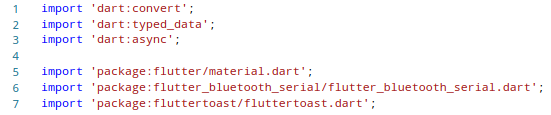
\includegraphics[height=2.5cm, width=12cm]{images/dart1}
     \captionof{figure}{Dart код - 1. део}
\end{center}
\indent\indentНа самом почетку се врши учитавање потребних библиотека. Најбитније су:
\begin{itemize}
    \item \texttt{material} - за исправно функционисање widget-a (графичких компоненти у оквиру апликације)
    \item \href{https://pub.dev/packages/flutter\_bluetooth\_serial}{\texttt{flutter\_bluetooth\_serial}} - за комуникацију са bluetooth модулом
    \item \texttt{fluttertoast} - омогућава испис Toast порука у оквиру апликације
\end{itemize}
\begin{center}
    \centering 
    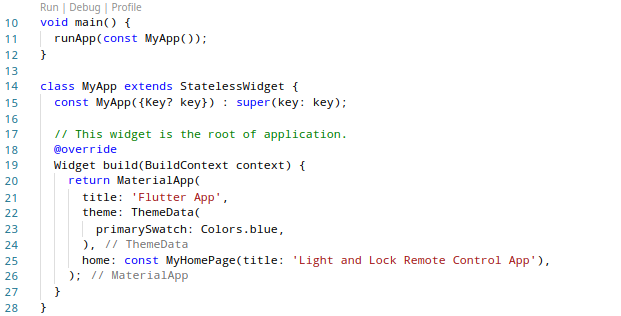
\includegraphics[height=8cm, width=14cm]{images/dart2}
     \captionof{figure}{Dart код - 2. део}
\end{center}
\indent\indentНакон учитавања библиотека позвали смо главну функцију \texttt{main()}. Унутар ње се позива уграђена функција \texttt{runApp} чији је аргумент објекат \texttt{MyApp} класе која је креирана испод и која наслеђује \texttt{StatelessWidget} уграђену класу. Унутар ње се предефинише \texttt{build} метода која се позива при креирању објекта класе и која враћа објекат типа \texttt{Widget}, а то ће у овом случају бити \texttt{MaterialApp} уграђени widget која ће бити на врху хијерархије осталих widget-а у апликацији. У оквиру њега налази се \texttt{MyHomePage} widget који представља почетну и једину страницу апликације у овом пројекту. 
\vspace{0.3cm}
\begin{center}
    \centering 
    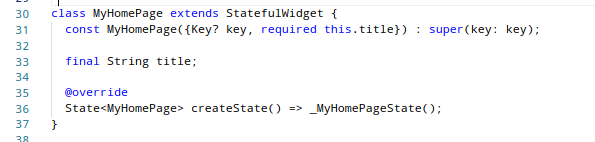
\includegraphics[height=4cm, width=14cm]{images/dart3}
     \captionof{figure}{Dart код - 3. део}
\end{center}
\indent\indentКласа \texttt{MyHomePage} наслеђује \texttt{StatefulWidget}. Разлика између \texttt{StatefulWidget} и \texttt{StatelessWidget} је та да се у \texttt{StatefulWidget}-у може динамички мењати садржај у току коришћења апликације што омогућава израду ефикаснијег и квалитетнијег корисничког интерфејса. Да би се имплементирало такво понашање потребно је да се предефинише уграђена функција \texttt{createState()} како би позвала објекат типа \texttt{State} који је у овом случају \texttt{\_MyHomePageState()}.
\vspace{0.3cm}
\begin{center}
    \centering 
    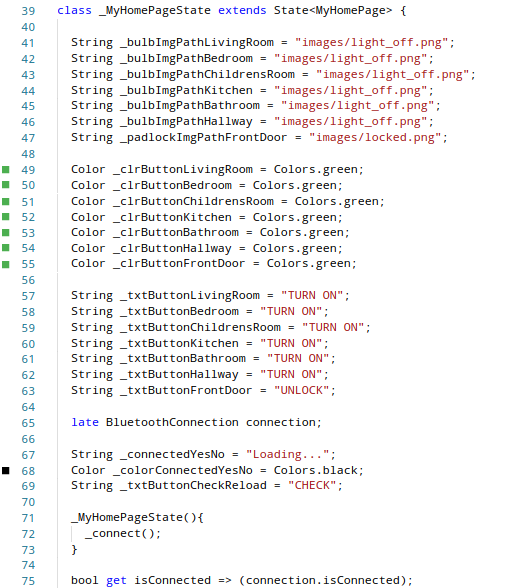
\includegraphics[height=17cm, width=14cm]{images/dart4}
     \captionof{figure}{Dart код - 4. део}
\end{center}
\indent\indentКласа \texttt{\_MyHomePageState} наслеђује \texttt{State} класу и садржи највећи део функционалности апликације. Све у наставку што садржи \texttt{main.dart} датотека јесте имплементација поменуте класе.\\
\indentНа самом почетку иницијализују се променљиве за путање слика, боје дугмади и текст дугмади на своје почетне вредности.\\
\indentЗатим се дефинише променљива \texttt{connection} типа \texttt{BluetoothConnection} која ће представљати објекат везе са bluetooth модулом. У конструктору класе се позива само функција \texttt{\_connect()} која ће бити објашњена у наставку. Променљива \texttt{isConnected} ће садржати логичку вредност да ли је веза остварена или не, тако што ће се у њу, када год се користи, сместити резултат позива функције \texttt{connection.isConnected}. 
\vspace{0.3cm}
\begin{center}
    \centering 
    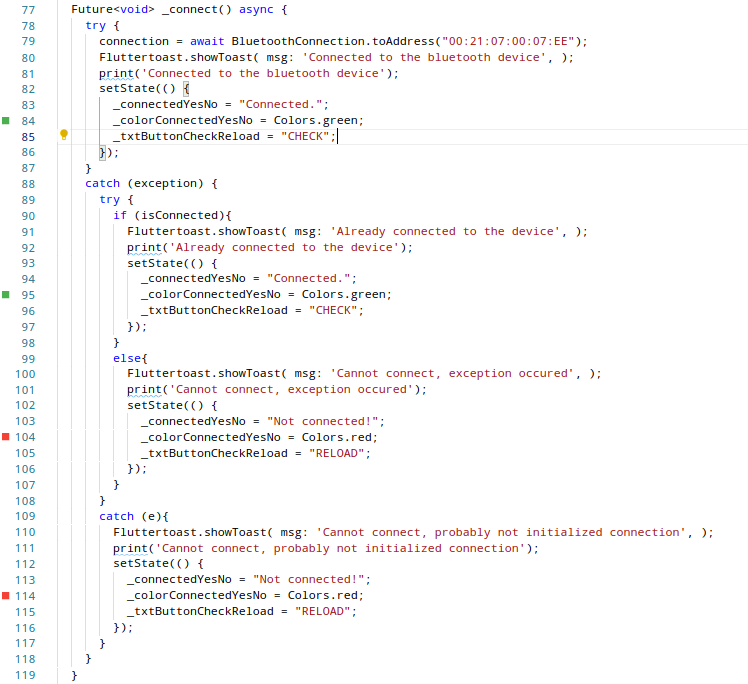
\includegraphics[height=18cm, width=16.5cm]{images/dart5}
     \captionof{figure}{Dart код - 5. део}
\end{center}
\indent\indentФункција \texttt{\_connect()} је функција у којој се иницијализује bluetooth веза тако што се се позива функција \texttt{toAddress} из класе \texttt{BluetoothConnection}. Њој је потребно да се проследи као аргумент MAC адреса уређаја на који се повезује, а то је у овом случају MAC адреса bluetooth модула и она је следећа: \texttt{00:21:07:00:07:EE}. Затим се корисник обавештава да је веза успостављена и подешава се динамички кориснички интерфејс тако што се позива уграђена функција \href{https://api.flutter.dev/flutter/widgets/State/setState.html}{\texttt{setState}} која се позива сваки пут када је потребно променити карактеристике неког widgeta-а динамички у току коришћења. У оквиру ње се реиницијализују променљиве које су коришћене од стране појединих widget-а да дефинишу одређене карактеристике. Такође, у оквиру функције \texttt{\_connect()} се хватају и одређени изузеци и то за случај да је корисник већ повезан, да се појавила грешка или да веза не може бити успостављена из разлога што неки од уређаја нема укључен bluetooth. Следи приказ графичког интерфејса ако је веза успостављена, ако није и ако покушава да се успостави:
\begin{figure}[H]
\centering
\subcaptionbox{Веза успостављена}{
\includegraphics[height=1cm, width=5cm]{images/conn1}}
\hfill % <-- Seperation
\subcaptionbox{Веза није успостављена}{
\includegraphics[height=1cm, width=5cm]{images/conn2}}
\hfill % <-- Seperation
\subcaptionbox{Веза покушава да се успостави}{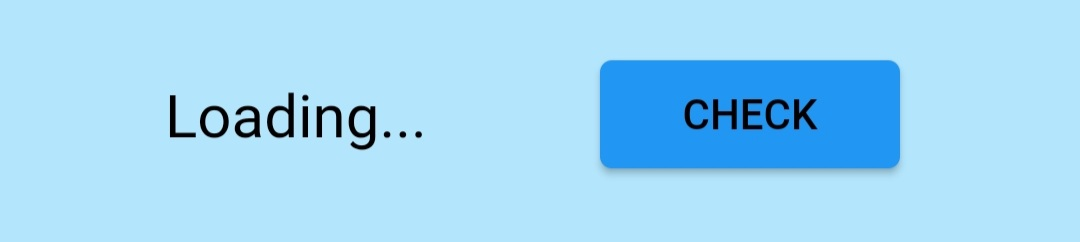
\includegraphics[height=1cm, width=5cm]{images/conn3}}
\caption{Приказ графичког интерфејса за различита стања bluetooth везе}
\end{figure}
\begin{center}
    \centering 
    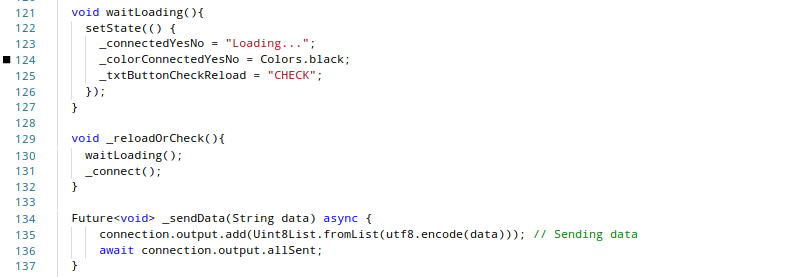
\includegraphics[height=8cm, width=18cm]{images/dart6}
     \captionof{figure}{Dart код - 6. део}
\end{center}
\indent\indentФункција \texttt{waitLoading} служи за подешавање графичких компоненти које се приказују док bluetooth веза покушава да се успостави. Унутар функције \texttt{\_reloadOrCheck} позивају се функције \texttt{waitLoading} и \texttt{\_connect} и служи да би уређај покушао поново да се повеже преко bluetooth-а или да провери постојећу bluetooth везу.\\
\indentНајбитнија од ових функција је \texttt{\_sendData} која као аргумент прима објекат типа \texttt{String}, а прослеђиваће јој се само један карактер који ће да служи као наредба коју прима bluetooth модул и прослеђује је микроконтролеру који слуша и извршава наредбе.
%\begin{center}
%    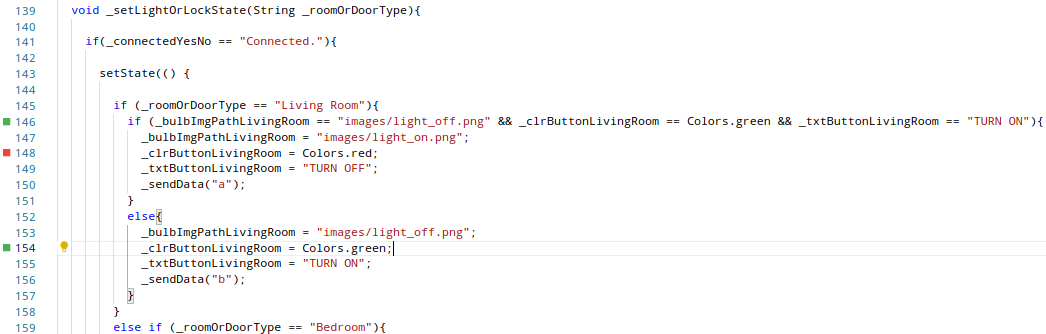
\includegraphics[height=7.5cm, width=17cm]{images/dart7}
%     \captionof{figure}{Dart код - 7. део}
%\end{center}
\begin{figure}[H]
\centering
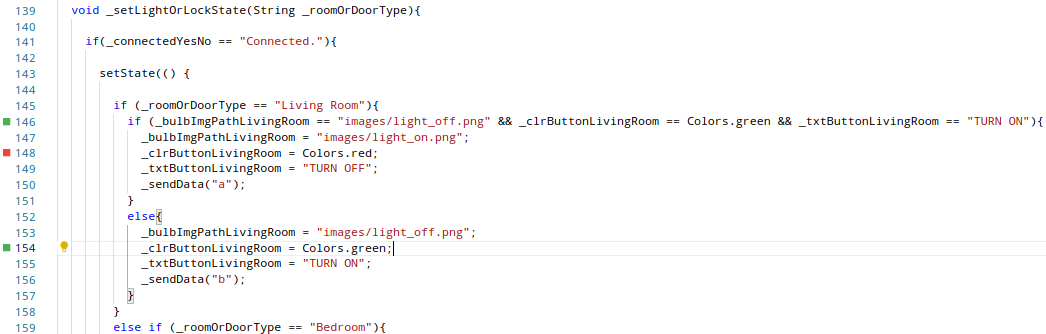
\includegraphics[height=7.5cm, width=17cm]{images/dart7}
\vspace{0.2cm}
\textbf{...}
\vspace{0.2cm}
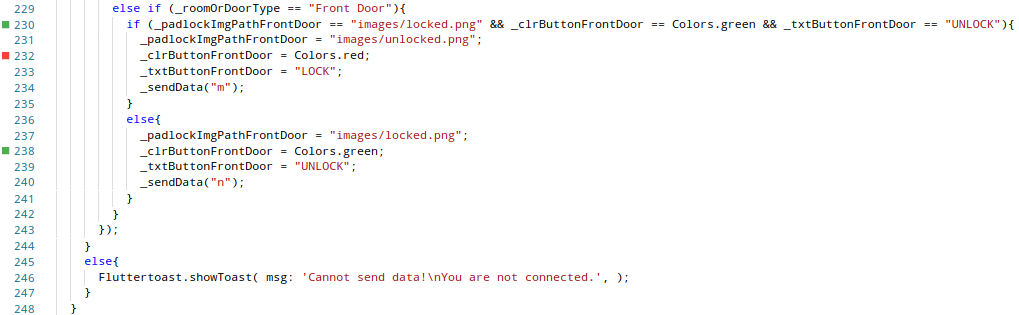
\includegraphics[height=7.5cm, width=17cm]{images/dart8}
\caption{Dart код - 7. део}
\end{figure}
\indent\indentФункција \texttt{\_setLightOrLockState} позива се кад год се притисне неко од дугмади TURN ON, TURN OFF, LOCK, UNLOCK у графичком корисничком интерфејсу. Као аргумент јој се прослеђује објекат типа \texttt{String} који представља назив просторије у којој се контролише осветљење или назив улаза на коме се врши контрола браве. На самом почетку унутар функције се проверава да ли је успостављена bluetooth веза и ако није корисник се о томе обавештава преко Toast поруке. Ако је веза успостављена позива се функција \texttt{setState} коју смо већ поменули. У оквиру њеног позива врши се провера који је \texttt{String} прослеђен функцији \texttt{\_setLightOrLockState} као аргумент. На слици изнад је приказан само случај када је у питању \texttt{'Living Room'}. Затим се проверава да ли вредности променљивих указују на то да је светло у тој просторији (у овом случају дневном боравку) искључено и ако јесте, те исте променљиве ће да добију вредности које указују на упаљено светло и доћи ће до промене у графичком корисничком интерфејсу, а такође се преко bluetooth везе шаље наредба 'a' која значи да светло треба да се упали. Промене у графичком корисничком интерфејсу су приказане на следећој слици:
\begin{figure}[H]
\centering
\subcaptionbox{Светло угашено}{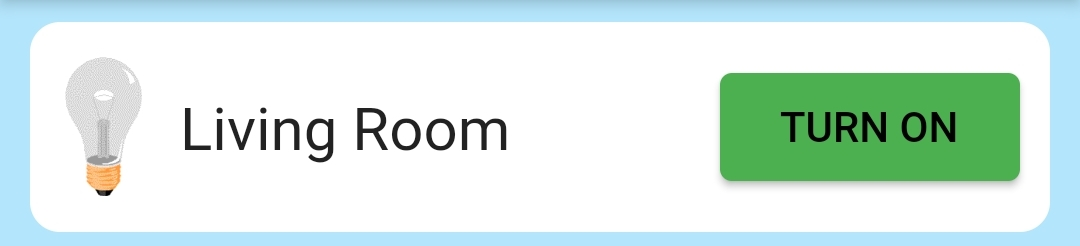
\includegraphics[height=1.5cm, width=7.5cm]{images/livingroomOFF}}
\hfill % <-- Seperation
\subcaptionbox{Светло упаљено}{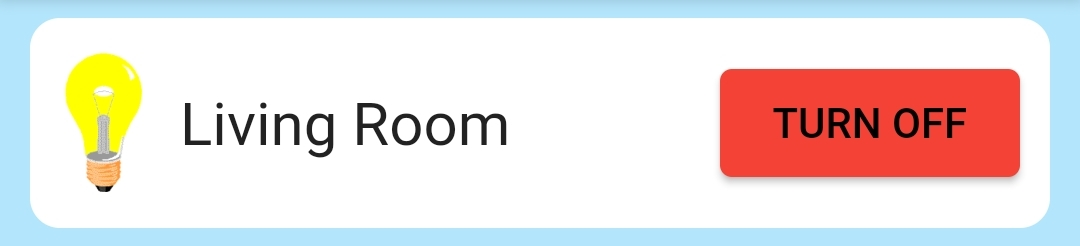
\includegraphics[height=1.5cm, width=7.5cm]{images/livingroomON}}
\caption{Изглед графичких компоненти за случај упаљеног и угашеног светла у дневном боравку}
\end{figure}
Ако променљиве не указују на то да је светло упаљено то значи да је светло угашено и да га треба упалити па се ради супротан процес, а преко bluetooth везе се шаље наредба 'b' која подразумева гашење светла. На слици изнад није приказан код за случај сваке просторије јер је логика иста као за случај дневног боравка. Оно што је битно напоменути јесте да се увек шаљу различите наредбе (карактери) преко bluetooth везе за сваку операцију посебно тј. ићи ће редом \texttt{a, b, c, d, ..., m, n}. На слици испод приказан је и случај ако је функцији \texttt{\_setLightOrLockState} као аргумент прослеђен стринг \texttt{'Front Door'} који подразумева контролу браве. За откључавање браве шаље се наредба 'm', а за закључавање наредба (податак, карактер) 'n'. Следи приказ графичких компоненти апликације за случај закључане и откључане браве:
\begin{figure}[H]
\centering
\subcaptionbox{Брава закључана}{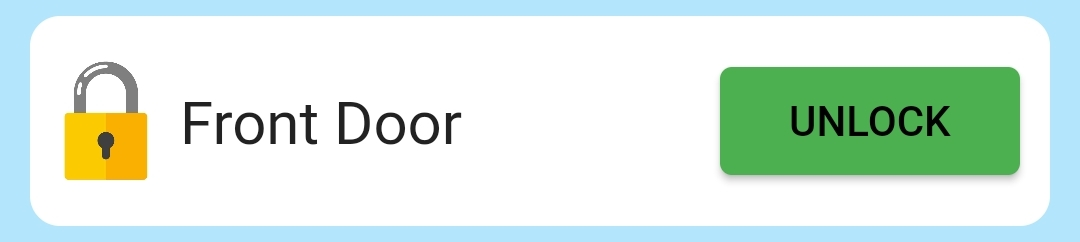
\includegraphics[height=1.5cm, width=7.5cm]{images/lckd}}
\hfill % <-- Seperation
\subcaptionbox{Брава откључана}{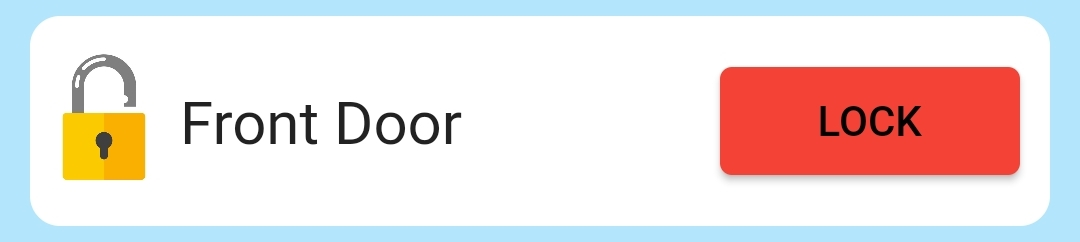
\includegraphics[height=1.5cm, width=7.5cm]{images/unlckd}}
\caption{Изглед графичких компоненти за случај закључане и откључане браве}
\end{figure}
\vspace{0.5cm}
\indent\indentНа слици испод је приказана импленемтација функције \texttt{\_buldRow} која враћа widget типа \texttt{Container} и служи да генерише графичке компоненте за један објекат којим се управља (брава, светло у свим просторијама посебно). Као аргументе јој је потребно проследити:
\begin{itemize}
    \item \texttt{String \_roomOrDoorType} - тип објекта којим ће се управљати тј. текст који ће бити исписан у средини widget-а.
    \item \texttt{String \_imagePath} - слика која ће бити смештена са леве стране widgeta-а \texttt{Container}.
    \item \texttt{Color \_clrButton} - боја дугмета које се налази унутар widget-а.
    \item \texttt{String \_txtButton} - текст лабела дугмета која указује на то коју акцију дугме извршава. 
\end{itemize}
\begin{center}
    \centering 
    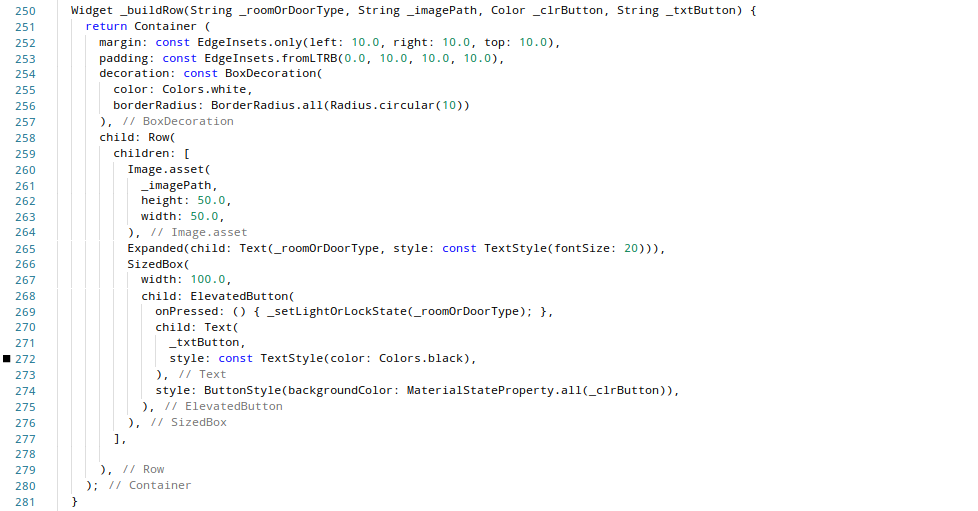
\includegraphics[height=13cm, width=20cm]{images/dart9}
     \captionof{figure}{Dart код - 8. део}
\end{center}
\vspace{0.3cm}
\indent\indentПр. Ако претходно приказану функцију позовемо на следећи начин:
\vspace{0.3cm}\\
\mycode{\_buildRow("Bedroom", \_bulbImgPathBedroom, \_clrButtonBedroom, \_txtButtonBedroom)}
\vspace{0.1cm}\\
тада ће се генерисати следећа графичка компонента (widget):
\begin{center}
    \centering 
    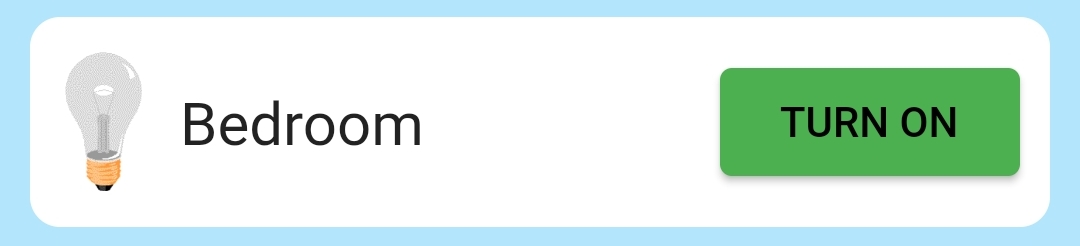
\includegraphics[height=1.5cm, width=7.5cm]{images/bedroomOFF}
     \captionof{figure}{\texttt{Container} widget за приказ једног предмета управљања - светлo у спаваћој соби}
\end{center}
\indent\indent\textbf{Напомена:} Још увек се налазимо у имплементацији класе \texttt{\_MyHomePageState}.\\\\
\indentУ наставку је приказана предефинисана функција \texttt{build} у оквиру класе \texttt{\_MyHomePageState} која враћа \texttt{Scaffold} widget који ће садржати главни део апликације тј. све оне графичке компоненте преко којих корисник може да управља хардверским компонентама и bluetooth везом.
\begin{center}
    \centering 
    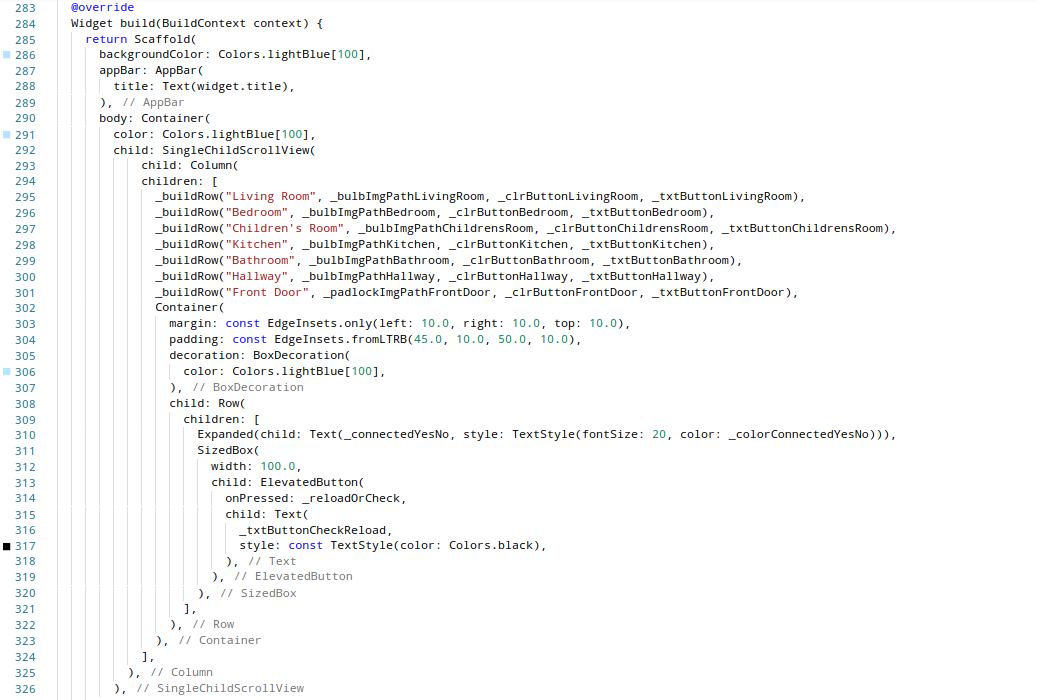
\includegraphics[height=17cm, width=21cm]{images/dart10}
     \captionof{figure}{Dart код - 9. део}
\end{center}
\indentОвим смо дошли до краја самог \texttt{main.dart} кода тј. имплементација мобилне апликације је завршена. 

\newpage
\section{Израда макете куће}
Макета куће која је потребна да би се употпунио прототип реалног система израђена је од комада шперплоче и изгледа као на следећим сликама:
\begin{figure}[H]
\centering
\includegraphics[height=8cm, width=12cm]{images/house1}
\vspace{0.5cm}\\
\includegraphics[height=5cm, width=7cm]{images/house2}
\hfill % <-- Seperation
\includegraphics[height=5cm, width=6cm]{images/house3}
\vspace{0.5cm}\\
\includegraphics[height=5cm, width=6cm]{images/house4}
\hfill % <-- Seperation
\includegraphics[height=5cm, width=7cm]{images/house5}
\caption{Изглед макете куће споља}
\end{figure}
\indentХардверске компоненте пројекта у оквиру макете куће налазе се на тавану и одатле су диоде и мотор спреведени на одговарајућа места. Кров макете може да се подигне како би се виделе хардверске компоненте које се налазе испод:
\begin{figure}[H]
\centering
\includegraphics[height=6.5cm, width=8cm]{images/house6}
\hfill % <-- Seperation
\includegraphics[height=6.5cm, width=8cm]{images/house7}
\caption{Положај хардверских компоненти на макети куће}
\end{figure}
\vspace{0.5cm}
\indentПлафон на коме се налазе хардверске компоненте такође може да се подигне да би се видео распоред просторија унутар макете куће. Направљене су преграде од шперплоче које имитирају више одвојених просторија: 
\vspace{0.2cm}
\begin{center}
    \centering 
    \includegraphics[height=9.8cm, width=14cm]{images/house8}
     \captionof{figure}{Распоред просторија унутар макете куће - поглед одозго}
\end{center}


\newpage
\section{Изглед и демонстрација рада апликације}
Мобилна апликација имплементирана у оквиру овог пројекта је једноставна са више компоненти које динамички мењају свој изглед у току коришћења. Следи приказ два screenshot-а покренуте апликације:
\begin{figure}[H]
\centering
\includegraphics[height=12cm, width=6cm]{images/app1}
\hfill % <-- Seperation
\includegraphics[height=12cm, width=6cm]{images/app2}
\caption{Изглед апликације након покретања и у току коришћења}
\end{figure}
\vspace{1cm}
\indent\textbf{ДЕМОНСТРАЦИЈА РАДА АПЛИКАЦИЈЕ:}\\ \indent\url{https://youtu.be/4k8WbcMCyuA}
\vspace{0.5cm}\\
\indent\textbf{Github страница пројекта:}\\
\indent\url{https://github.com/djoto/Flutter-Arduino_light_and_lock_bluetooth_control}

\newpage
\section{Литература}
\begin{itemize}
  \item The Arduino Projects Book, Scott Fitzgerald and Michael Shiloh,  Torino, Italy, September 2012
  \item \url{http://moodle.fink.rs/pluginfile.php/36385/mod\_resource/content/1/PMA\%20-\%20Dokumentacija.pdf} - ПМА Документација, Бобан Срећковић, Крагујевац 2019
  \item \url{http://ww1.microchip.com/downloads/en/DeviceDoc/Atmel-7810-Automotive-Microcontrollers-ATmega328P\_Datasheet.pdf} - ATmega328P спецификација
  \item \url{https://components101.com/sites/default/files/component\_datasheet/HC-05\%20Datasheet.pdf} - HC-05 спецификација
  \item \url{http://www.ee.ic.ac.uk/pcheung/teaching/DE1\_EE/stores/sg90\_datasheet.pdf} - Micro Servo SG90 спецификација
  \item \url{https://en.wikipedia.org/wiki/Light-emitting_diode}
  \item \url{https://www.arduino.cc/en/software}
  \item \url{https://en.wikipedia.org/wiki/C\_(programming_language}
  \item \url{https://en.wikipedia.org/wiki/Flutter\_(software)}
  \item \url{https://en.wikipedia.org/wiki/Dart\_(programming\_language)}
  \item \url{https://docs.flutter.dev/get-started/install}
  \item \url{https://code.visualstudio.com/}
  \item \url{https://docs.flutter.dev/get-started/editor?tab=vscode}
  \item \url{https://en.wikipedia.org/wiki/LaTeX}
  \item \url{https://www.latex-project.org/get/}
  \item \url{https://www.overleaf.com/project}
  \item \url{https://www.tinkercad.com/dashboard}
  \item \url{https://easyeda.com/}
  \item \url{https://www.arduino.cc/en/Reference/softwareSerial}
  \item \url{https://www.arduino.cc/reference/en/libraries/servo/}
  \item \url{https://en.wikipedia.org/wiki/Baud}
  \item \url{https://www.arduino.cc/reference/en/language/functions/math/map/}
  \item \url{https://docs.flutter.dev/get-started/test-drive?tab=vscode}
  \item \url{https://pub.dev/packages/flutter\_bluetooth\_serial}
  \item \url{https://api.flutter.dev/flutter/widgets/State/setState.html}
  \item \url{https://stackoverflow.com/}
  \item \url{https://youtu.be/4k8WbcMCyuA} - YouTube линк демонстрације рада апликације
  \item \url{https://github.com/djoto/Flutter-Arduino_light_and_lock_bluetooth_control} - Github страница пројекта
\end{itemize}


\end{document}
